\begin{figure*}[tp]
\centering
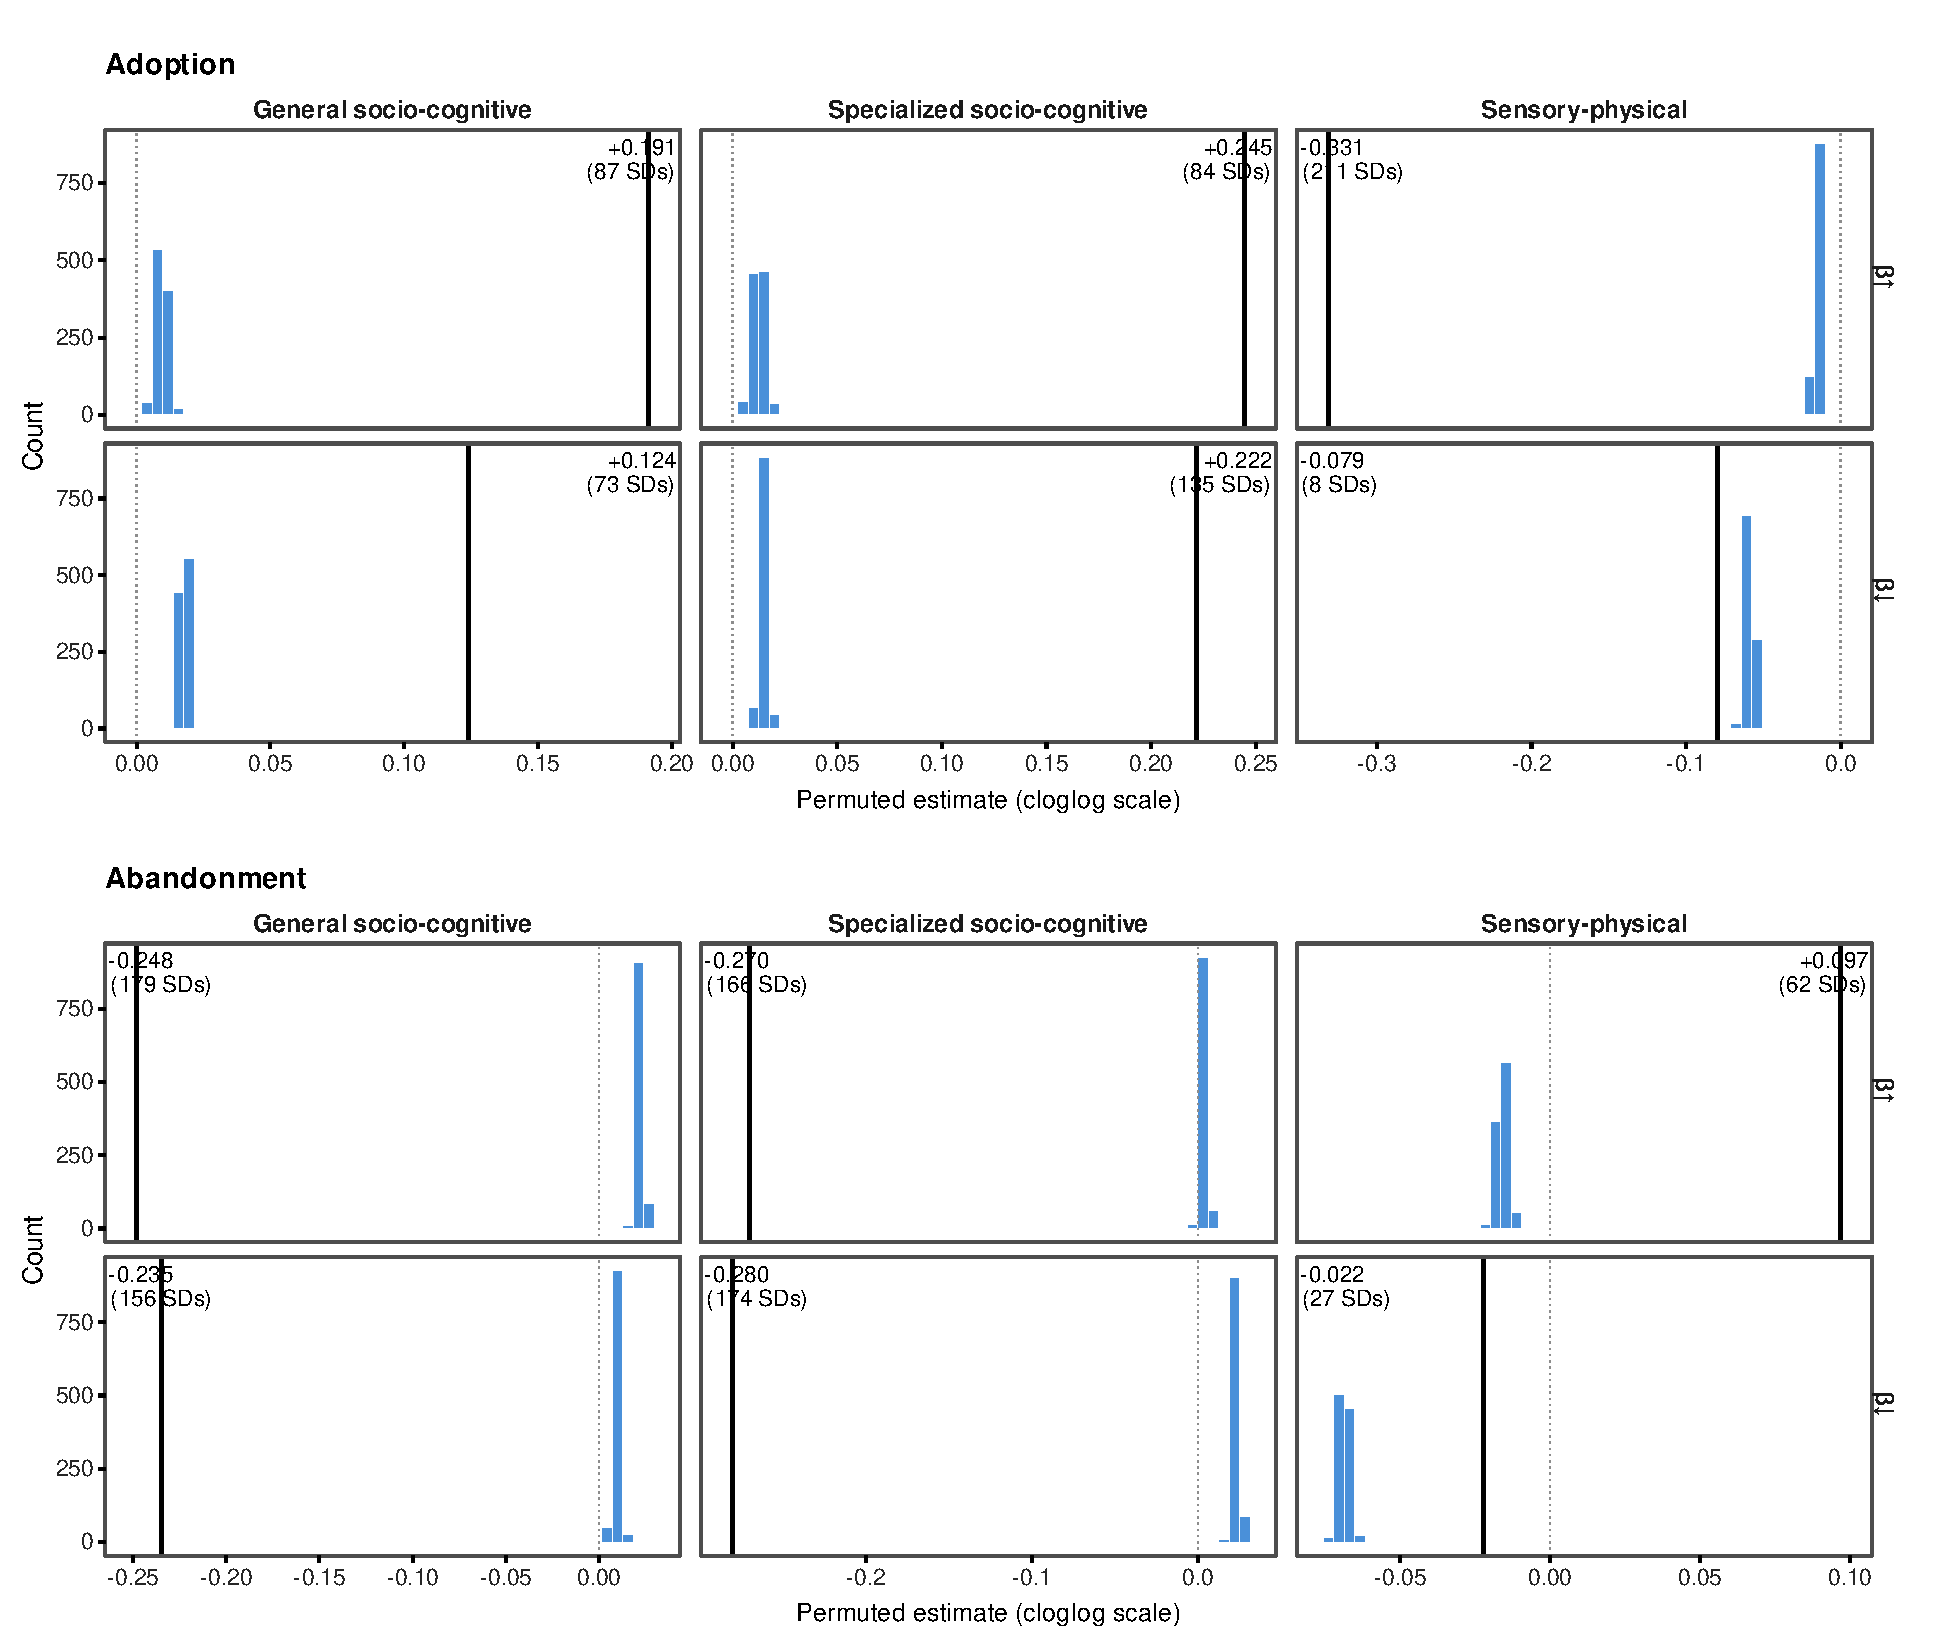
\includegraphics[width=0.95\textwidth]{figures/fig_SI_test_iii.pdf}
\caption{\textbf{Observed coefficients are far outside the within-stratum permutation null.} Each histogram shows the distribution of $B = 1{,}000$ permuted estimates, where the outcome is randomly reassigned within cells defined by skill type $\times$ source status quintile. The vertical line marks the observed Panel~A estimate; the annotation reports the observed value and its distance from the null in null standard deviations. Rows correspond to $\hat{\beta}^{\uparrow}$ (top) and $\hat{\beta}^{\downarrow}$ (bottom); columns to skill type. All twelve observed coefficients fall outside the null distribution ($p < 0.001$), inconsistent with correlated technological shocks as the primary driver of the directional asymmetry. O*NET 2015--2024. \textbf{(A)} Adoption. \textbf{(B)} Abandonment.}
\label{fig:SI_test_iii}
\end{figure*}
